\documentclass[11 pt]{article}
\usepackage{graphicx}
%\usepackage{mysty}
%\usepackage{amsmath}
\usepackage{url}

\begin{document}

\section*{Computerized Mechanical Resonance Experiments}

Build a resonance system using available resources.
Using LabVIEW or Python, sweep through drive frequencies and measure the amplitude and phase response of the system.

\begin{figure}[h]
	\begin{center}
		\includegraphics[width=5in]{device}
	\end{center}
	\caption{Mechanical computer-controlled driver}
	\label{fig:driver}
\end{figure}

\subsection*{Too-Simple Example}

Connect two Vernier GoDirect Sensor Carts (i.e. 204A carts) with three springs and the SinDrive device:

driver --spring-- cart 1 --spring-- cart 2 --spring-- track endstop.

Write a Python program that sweeps through an appropriate range of drive frequencies and uses the Vernier GoDirect Python library to measure cart position/time data at that frequency. 
Use the numpy.fft library to calculate the amplitude and phase of the cart motion, relative to the drive phase.
Use this data to make a plot such as figure \ref{fig:2-carts}.

\begin{figure}[h]
	\begin{center}
		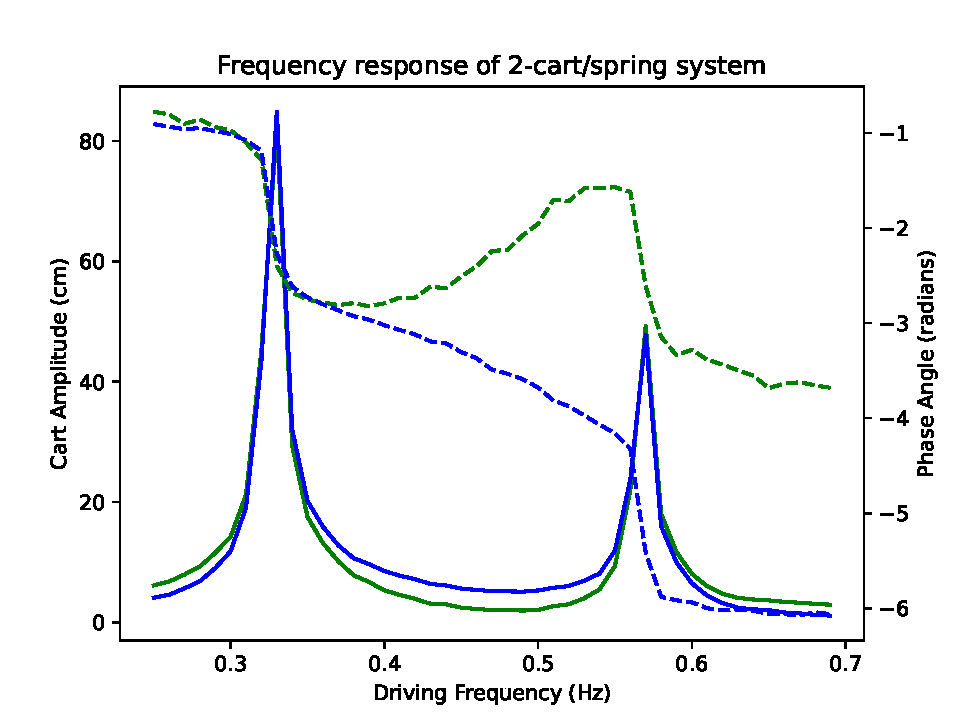
\includegraphics[width=5in]{2-cart_response}
	\end{center}
	\caption{Amplitude(solid lines) and phase (dashed lines) for two coupled carts}
	\label{fig:2-carts}
\end{figure}

\subsection*{Resources}
\begin{itemize}
	\item Dr. Ayars's CartDriver library: \url{https://github.com/EricAyars/Cart-driver/tree/main/AdvLab}
		This library provides a simple object-oriented API for controlling everything about the SinDrive apparatus.
		Example usage is included in CartDriver.py
	\item Vernier Software provides an API for all of their GoDirect sensors, including carts:\url{https://www.vernier.com/engineering/python/}. You will need to install the godirect library on your python installation (pip install godirect). 
		Once that's done, it's easiest to use the godirect library from within the GDX wrapper, a copy of which is available either from Vernier Software or on the Ayars GitHub repo.
	\item Sample code ---the code Dr. Ayars used to make the graph above--- is given in AutoResonance.py on GitHub.
\end{itemize}

\subsection*{Ideas}
Here are some ideas for this experiment that as of Fall '25 haven't been done yet:
\begin{itemize}
	\item Hang a Vernier cart from a spring attached to the SinDrive and look at the relationship between driven vertical motion and rotational/vertical oscillations.
	\item Put two spring-coupled carts on a track, but instead of a horizontal track make the track nearly vertical. 
		Calculate (predict) the resonant frequencies and the relative motions of the carts, then match to experiment.
	\item Three coupled carts. 
		Calculate resonant frequencies and `shapes' of the normal modes, match to experiment.
	\item Normal modes with unequal masses.
	\item From the width of the resonance, calculate the damping coefficient for a cart
	\item The carts can measure Force, Acceleration on three axes, Angular Velocity on three axes, and Position. Use your imagination and think of interesting experiments.
\end{itemize}

\end{document}

